\documentclass{beamer}

\newif\ifmacron
\macrontrue

\usepackage[T1]{fontenc}
\usepackage{../unicode}
\usepackage[american]{babel}
\usepackage{amsmath,amssymb,amsthm}
\usepackage{tikz,pgflibraryarrows,pgflibraryplotmarks,pgflibrarysnakes,pgflibraryshapes}
\usepackage{tikzsymbols}
\usepackage[backend=biber,citestyle=authoryear-comp,bibstyle=beamer,doi=false,isbn=false,url=false,maxnames=10]{biblatex}
\usepackage[nosfdefault]{comicneue}
\usepackage[normalem]{ulem}
\bibliography{../isogenies_bib/isogenies,../hdr}

\mode<presentation>{%
  \usetheme{Boadilla}
}
\beamertemplatenavigationsymbolsempty

\usepackage{sourcesanspro}
\usepackage[amssymb,amsfonts]{concmath}
\usefonttheme[onlymath]{serif}

\renewcommand{\emph}[1]{{\usebeamercolor[fg]{structure}#1}}

%\let\footcite\footnote

\RequirePackage{amsmath,amsfonts}

\DeclareMathOperator{\End}{End}
\DeclareMathOperator{\Tr}{Tr}
\DeclareMathOperator{\Gal}{Gal}
\DeclareMathOperator{\ord}{ord}
\DeclareMathOperator{\loglog}{loglog}
\DeclareMathOperator{\GL}{GL}
\DeclareMathOperator{\SL}{SL}
\DeclareMathOperator{\Cl}{Cl}

\def\R{\ensuremath{\mathbb{R}}}
\def\A{\ensuremath{\mathbb{A}}}
\def\P{\ensuremath{\mathbb{P}}}
\def\F{\ensuremath{\mathbb{F}}}
\def\O{\ensuremath{\mathcal{O}}}
\def\tildO{\ensuremath{\tilde{O}}}
\def\euler{\ensuremath{\varphi}}

% \newcommand{\C}{\mathbb{C}}
% \newcommand{\R}{\mathbb{R}}
% \newcommand{\Z}{\mathbb{Z}}
% \newcommand{\N}{\mathbb{N}}
% \newcommand{\Q}{\mathbb{Q}}
% \newcommand{\F}{\mathbb{F}}
% \renewcommand{\O}{\mathcal{O}}
% \newcommand{\tildO}{\mathcal{\tilde{O}}}
% \newcommand{\End}{\operatorname{End}}
% \newcommand{\chr}{\operatorname{char}}
% \newcommand{\Cl}{\operatorname{Cl}}
% \renewcommand{\a}{{\mathfrak{a}}}
% \renewcommand{\b}{{\mathfrak{b}}}
% \newcommand{\cyc}[1]{{\langle #1 \rangle}}
% \newcommand{\ord}{\operatorname{ord}}

\usetikzlibrary{matrix,decorations,decorations.text,calc,arrows,snakes,shapes,positioning}

% \pgfkeys{/triangle/.code=\tikzset{x={(-0.5cm,-0.866cm)},y={(1cm,0cm)}}}
% \pgfkeys{/lattice/.code n args={4}{\tikzset{cm={#1,#2,#3,#4,(0,0)}}}}

% \newcommand{\axes}[4]{
%   \clip (#1,#3) rectangle (#2,#4);
%   \draw [thin, gray, -latex] (#1,0) -- (#2,0);% Draw x axis
%   \draw [thin, gray, -latex] (0,#3) -- (0,#4);% Draw y axis
% }

% \newcommand{\lattice}[2]{
%   \draw[style=help lines,dashed] (#1-1,#1-1) grid[step=1] (#2+1,#2+1);
%   \foreach \x in {#1,...,#2}{
%     \foreach \y in {#1,...,#2}{
%       \node[draw,circle,inner sep=2pt,fill] at (\x,\y) {};
%       % Places a dot at those points
%     }
%   }
% }

% % This command defines a triangle of dots of given height
% \newcommand{\dottriangle}[2][\i-\j]{%
%   \foreach \i in {0,...,#2} {%
%     \foreach \j in {0,...,\i} {%
%       \draw(\i,\j) node{#1};%
%     }%
%   }}


\title[Exploring Isogeny Graphs]{Exploring Isogeny Graphs\\
  \normalsize Around the Volcano in $2^{80}$ Days}
\author[Luca De Feo]{Luca De Feo\\
  \small hand drawings by Rachel Deyts}
\date{Dec 14, 2018, UVSQ, Versailles}
\institute[UVSQ]{Université Paris Saclay -- UVSQ}

\begin{document}

\frame[plain]{\titlepage}

%%

% 1. Elliptic curve. It is a group. Drawing.

\begin{frame}{Elliptic curves}

  Let \emph{$E \;:\; y^2 = x^3 + ax + b$} be an elliptic curve\dots

  \begin{columns}
    \begin{column}{0.35\textwidth}
      \begin{itemize}
      \item An algebraic curve,
      \item<2-> A group.
      \end{itemize}
    \end{column}
    \begin{column}{0.65\textwidth}
      \begin{tikzpicture}[domain=-2.4566:4,samples=100]
        \begin{scope}
          \draw plot (\x,{0.5*sqrt(\x*\x*\x-4*\x+5)});
          \draw plot (\x,{-0.5*sqrt(\x*\x*\x-4*\x+5)});
        \end{scope}

        \begin{scope}[yscale=1/2]
          \draw[thin,gray,-latex] (0,-7) -- (0,7);
          \draw[thin,gray,-latex] (-3,0) -- (4,0);
          
          \begin{uncoverenv}<2->
            \draw (-3,1) -- (4,8/3+3);
            \begin{scope}[every node/.style={draw,circle,inner sep=1pt,fill},cm={1,2/3,0,0,(0,3)}]
              \node at (-2.287980,0) {};
              \node at (-0.535051,0) {};
              \node at (3.267475,0) {};
            \end{scope}
            \begin{scope}[every node/.style={yshift=0.3cm},cm={1,2/3,0,0,(0,3)}]
              \node at (-2.287980,0) {$P$};
              \node at (-0.535051,0) {$Q$};
              \node at (3.267475,0) {$R$};
            \end{scope}
            \draw[dashed] (3.267475,3.267475*2/3+3) -- (3.267475,-3.267475*2/3-3) 
            node[draw,circle,inner sep=1pt,fill] {}
            node[xshift=-0.1cm,anchor=east] {$P+Q$};
          \end{uncoverenv}
        \end{scope}
      \end{tikzpicture}
    \end{column}
  \end{columns}
\end{frame}

% 2. Why does CS care? DH (insist prime order). But also ECM, ECPP, etc.

\ifmacron
{
  \setbeamercolor{background canvas}{bg=black}
  \setbeamercolor{frametitle}{fg=white!70!black}
  \begin{frame}[plain]
    \frametitle{What do you think, startup nation?}
    
    \begin{tikzpicture}[remember picture,overlay]
      \large\bf
      \node(pic)[at=(current page.center),yshift=-0.5cm] {
        \includegraphics[width=\paperwidth]{macron-perplexe.jpg}
      };
    \end{tikzpicture}
  \end{frame}
}
\fi

%%

\begin{frame}{Why should I care? (Diffie--Hellman key exchange)}
  \begin{description}
  \item[Goal:] Alice and Bob have never met before. They are chatting
    over a public channel, and want to agree on a \emph{shared secret}
    to start a private conversation.
  \item[Setup:] They agree on a (large) cyclic group $E(\F_p)=〈P〉$
    of (prime) order $q$.
  \end{description}

  \begin{center}
    \begin{tikzpicture}
      \node at (0,0) {\bf Alice};
      \node at (7,0) {\bf Bob};
      \node at (0,-1) {pick random \alert{$a∈ℤ/qℤ$}};
      \node at (0,-1.5) {compute $A=[a]P$};
      \node at (7,-1) {pick random \alert{$b∈ℤ/qℤ$}};
      \node at (7,-1.5) {compute $B=[b]P$};
      \draw[->]
      (1,-2) to node[auto] {$A$} (6,-2);
      \draw[->] (6,-2.5) to node[auto] {$B$} (1,-2.5);
      \node at (3.5,-3.5) {\emph{Shared secret} is \alert{$[a]B=[ab]P=[b]A$}};
    \end{tikzpicture}
  \end{center}
\end{frame}

%%

\begin{frame}{Why should I care?}

  {\large\emph{But, also:}}
  \begin{itemize}
  \item Elliptic Curve Factoring Method (Lenstra '85);
  \item Elliptic Curve Primality Proving (Atkin, Morain '86-'93);
  \item Efficient normal bases for finite fields (Couveignes, Lercier '10);
  \item \dots
  \end{itemize}
\end{frame}

%% 

\begin{frame}{Why should I care?}
  \begin{center}
    \begin{tikzpicture}[domain=-2.4566:4,samples=100]
      \newcount\rotate
      \animate<2-6>
      \animatevalue<2-6>{\rotate}{0}{90}
      \begin{scope}[rotate=-\the\rotate]
        \draw plot (\x,{0.5*sqrt(\x*\x*\x-4*\x+5)});
        \draw plot (\x,{-0.5*sqrt(\x*\x*\x-4*\x+5)});
      \end{scope}
      
      \begin{uncoverenv}<1>
        \begin{scope}[yscale=1/2]
          \draw[thin,gray,-latex] (0,-7) -- (0,7);
          \draw[thin,gray,-latex] (-3,0) -- (4,0);
          
          \draw (-3,1) -- (4,8/3+3);
          \begin{scope}[every node/.style={draw,circle,inner sep=1pt,fill},cm={1,2/3,0,0,(0,3)}]
            \node at (-2.287980,0) {};
            \node at (-0.535051,0) {};
            \node at (3.267475,0) {};
          \end{scope}
          \begin{scope}[every node/.style={yshift=0.3cm},cm={1,2/3,0,0,(0,3)}]
            \node at (-2.287980,0) {$P$};
            \node at (-0.535051,0) {$Q$};
            \node at (3.267475,0) {$R$};
          \end{scope}
          \draw[dashed] (3.267475,3.267475*2/3+3) -- (3.267475,-3.267475*2/3-3) 
          node[draw,circle,inner sep=1pt,fill] {}
          node[xshift=-0.1cm,anchor=east] {$P+Q$};
        \end{scope}
      \end{uncoverenv}
    \end{tikzpicture}
  \end{center}
\end{frame}

%%

\begin{frame}{Elliptic curves}
  \transdissolve
  \centering
  
\includegraphics[height=0.7\textheight]{ec-happy}

  \Large\bf I power 70\% of WWW traffic!
\end{frame}

%%

\ifmacron
{
  \setbeamercolor{background canvas}{bg=black}
  \setbeamercolor{frametitle}{fg=white!70!black}
  \begin{frame}[plain]
    \begin{tikzpicture}[remember picture,overlay,white]
      \large\bf
      \node(pic)[at=(current page.center)] {
        \includegraphics[width=\paperwidth]{macron-pollice.jpg}
      };
    \end{tikzpicture}
  \end{frame}
}
\fi

% 3. What is scalar mul -> an isogeny?

\begin{frame}{What is \alt<2->{\xout{scalar multiplication} an
      isogeny}{scalar multiplication}?}

  \begin{overlayarea}{\textwidth}{4em}
    \Large
    \[
      \alt<3->{ϕ}{[n]}
      \;:\; P \mapsto
      \alt<3->{ϕ(P)}{\underbrace{P + P + \cdots + P}_{n\text{ times}}}\]
  \end{overlayarea}
  
  \begin{itemize}
  \item A map \emph{$E\to \alt<4->{\xout{E} E'}{E\phantom{\xout{}}}$},
  \item a \emph{group morphism},
  \item with \emph{finite kernel}\\
    \alt<5->{(\xout{the torsion group $E[n]≃(ℤ/nℤ)^2$} any
      finite subgroup \emph{$H\subset E$})}{(the torsion group
      \emph{$E[n]\simeq(ℤ/nℤ)^2$})},
  \item \emph{surjective} (in the algebraic closure),
  \item given by \emph{rational maps} of degree \alt<6->{\xout{$n^2$}
      \emph{$\#H$}}{\emph{$n^2$}}.
  \end{itemize}

  \begin{uncoverenv}<7->
    (Separable) isogenies $⇔$ finite subgroups:
    \alert{\[0 → H → E \overset{ϕ}{→} E' \to 0\]}
    The kernel \emph{$H$} determines the image curve \emph{$E'$} up to
    isomorphism \[\emph{E/H\overset{\text{\tiny def}}{=}E'}.\]
  \end{uncoverenv}
\end{frame}

% 4. example

\begin{frame}{Isogenies: an example over $\F_{11}$}
  \begin{tikzpicture}[scale=0.4]
    \begin{scope}
      \node[anchor=center] at (0,7) {$E \;:\; y^2 = x^3 + x$};

      \uncover<-1>{
        \draw[thin,gray] (0,-6) -- (0,6);
        \draw[thin,gray] (-6,0) -- (6,0);
      }

      \foreach \x/\y in {0/0,5/3,-4/3,-3/5,-2/1,-1/3} {
        \draw[blue,fill] (\x,\y) circle (0.2) node(E_\x_\y){}
        (\x,-\y) circle (0.2) node(E_\x_-\y){};
      }

      \uncover<2->{\draw[red,fill] (0,0) circle (0.3);}
    \end{scope}

    \draw[black!10!white,thick] (8,-7) -- +(0,14);
    
    \begin{scope}[shift={(16,0)}]
      \node at (0,7) {$E' \;:\; y^2 = x^3 - 4x$};

      \uncover<-1>{
        \draw[thin,gray] (0,-6) -- (0,6);
        \draw[thin,gray] (-6,0) -- (6,0);
      }

      \foreach \x/\y in {0/0,2/0,3/2,4/2,6/4,-2/0,-1/5} {
        \draw[color=blue,fill] (\x,\y) circle (0.2) node(F_\x_\y){}
        (\x,-\y) circle (0.2) node(F_\x_-\y){};
      }
    \end{scope}

    \begin{scope}[color=red,-latex,dashed]
      \begin{uncoverenv}<2->
        \path
        (E_5_3) edge (F_3_2)
        (E_-4_3) edge (F_4_-2)
        (E_-3_5) edge (F_4_2)
        (E_-2_1) edge (F_3_-2)
        (E_-1_3) edge (F_-2_0);
      \end{uncoverenv}
      \begin{uncoverenv}<2->
        \path
        (E_5_-3) edge (F_3_-2)
        (E_-4_-3) edge (F_4_2)
        (E_-3_-5) edge (F_4_-2)
        (E_-2_-1) edge (F_3_2)
        (E_-1_-3) edge (F_-2_0);
      \end{uncoverenv}
    \end{scope}
  \end{tikzpicture}
  
  \begin{columns}
    \begin{column}{0.5\textwidth}
      \[ϕ(x,y) = \left(\frac{x^2 + 1}{x},\quad y\frac{x^2-1}{x^2}\right)\]
    \end{column}
    \begin{column}{0.5\textwidth}
      \begin{itemize}
      \item<2-> Kernel generator in \alert{red}.
      \item<2-> This is a degree $2$ map.
      \item<2-> Analogous to $x↦x^2$ in $\F_q^*$.
      \end{itemize}
    \end{column}
  \end{columns}
\end{frame}

% 5. Isogeny computations. Why? SEA, explicit isogeny, Vélu, other problems.

\begin{frame}{Computing Isogenies}
  \begin{block}{Vélu's formulas}
    \begin{description}
    \item[Input:] A subgroup \emph{$H⊂E$},
    \item[Output:] The isogeny \emph{$ϕ:E→E/H$}.
    \item[Complexity:] \emph{$O(ℓ)$} --- \cite{velu71}, \dots
    \item[Why?]
      \begin{itemize}
      \item Evaluate isogeny on points \emph{$P∈E$};
      \item Walk in \emph{isogeny graphs}.
      \end{itemize}
    \end{description}
  \end{block}

  \pause
  
  \begin{block}{Explicit Isogeny Problem}
    \begin{description}
    \item[Input:] Curve \emph{$E$}, (prime) integer \emph{$ℓ$}
    \item[Output:] All subgroups \emph{$H⊂E$} of order
      \emph{$ℓ$}.
    \item[Complexity:] \emph{$\tildO(ℓ^2)$} --- \cite{elkies92}
    \item[Why?]
      \begin{itemize}
      \item List all isogenies of given degree;
      \item Count points of elliptic curves;
      \item Compute endomorphism rings of elliptic curves;
      \item Walk in \emph{isogeny graphs}.
      \end{itemize}
    \end{description}
  \end{block}
\end{frame}

%%

\begin{frame}{Computing Isogenies}
  \begin{block}{Explicit Isogeny Problem (2)}
    \begin{description}
    \item[Input:] Curves \emph{$E,E'$}, isogenous of degree \emph{$ℓ$}.
    \item[Output:] The isogeny \emph{$ϕ:E→E'$} of degree \emph{$ℓ$}.
    \item[Complexity:] \emph{$O(ℓ^2)$} ---
      \cite{elkies92,couveignes96,lercier+sirvent08,df10,defeo2016explicit,lairez-vaccon}, \dots
    \item[Why?]
      \begin{itemize}
      \item Count points of elliptic curves.
      \end{itemize}
    \end{description}
  \end{block}

  \pause
  
  \begin{block}{Isogeny Walk Problem}
    \begin{description}
    \item[Input:] Isogenous curves \emph{$E,E'$}.
    \item[Output:] An isogeny \emph{$ϕ:E→E'$} of \emph{smooth} degree.
    \item[Complexity:] Generically hard --- \cite{GHS}, \dots
    \item[Why?]
      \begin{itemize}
      \item Cryptanalysis (ECC);
      \item Foundational problem for \alert{isogeny-based cryptography}.
      \end{itemize}
    \end{description}
  \end{block}
\end{frame}

\ifmacron
{
  \setbeamercolor{background canvas}{bg=black}
  \setbeamercolor{frametitle}{fg=white!70!black}
  \begin{frame}[plain]
    \begin{tikzpicture}[remember picture,overlay,white]
      \large\bf
      \node(pic)[at=(current page.center)] {
        \includegraphics[width=0.9\paperwidth]{macron-suffering.jpg}
      };
    \end{tikzpicture}
  \end{frame}
}
\fi

% 7. isogeny graphs. Why? Exploring

\begin{frame}
  \frametitle{Isogeny graphs}
  
  \vspace{-2mm}

  \begin{columns}
    \begin{column}{0.65\textwidth}
      We look at the graph of elliptic curves with isogenies \emph{up
        to isomorphism}.  We say two \alert{isogenies} $ϕ,ϕ'$
      are \alert{isomorphic} if:
    \end{column}
    \begin{column}{0.3\textwidth}
      \begin{center}
        \begin{tikzpicture}[node distance=4em]
          \node(E){$E$}; 
          \node(E1)[right of=E]{$E'$};
          \node(E2)[below of=E1]{$E'$};
          \scriptsize
          \path[->] (E) edge node[auto]{$ϕ$} (E1);
          \path[->] (E) edge node[auto,swap]{$ϕ'$} (E2);
          \path[<->] (E1) edge node[rotate=270] {\large$\widetilde{}$} (E2);
        \end{tikzpicture}
      \end{center}
    \end{column}
  \end{columns}

  \emph{Example:} Finite field, ordinary case, graph of isogenies of degree $3$.

  \begin{center}
    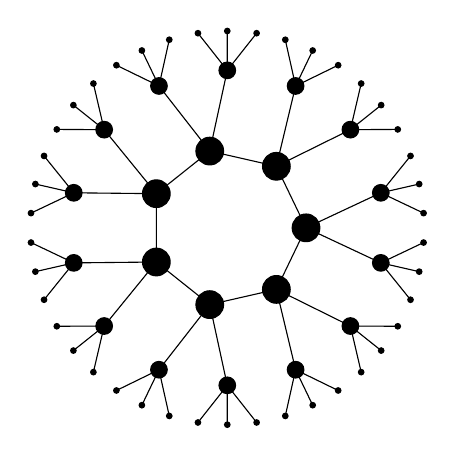
\begin{tikzpicture}[]
      \begin{scope}
        \def\crater{7}
        \foreach \i in {1,...,\crater} {
          \draw[fill] (360/\crater*\i:1cm) circle (5pt);
          \draw (360/\crater*\i : 1cm) -- (360/\crater*\i+360/\crater : 1cm);
          \foreach \j in {-1,1} {
            \draw[fill] (360/\crater*\i : 1cm) -- (360/\crater*\i + \j*360/\crater/4 : 2cm) circle (3pt);
            \foreach \k in {-1,0,1} {
              \draw[fill] (360/\crater*\i + \j*360/\crater/4 : 2cm) --
              (360/\crater*\i + + \j*360/\crater/4 + \k*360/\crater/6 : 2.5cm) circle (1pt);
            }
          }
        }
      \end{scope}
    \end{tikzpicture}
  \end{center}
\end{frame}

%%

\ifmacron
{
  \setbeamercolor{background canvas}{bg=black}
  \setbeamercolor{frametitle}{fg=white!70!black}
  \begin{frame}[plain]
    \begin{tikzpicture}[remember picture,overlay,white]
      \large\bf
      \node(pic)[at=(current page.center)] {
        \includegraphics[height=\paperheight]{macron-angry.jpg}
      };
    \end{tikzpicture}
  \end{frame}
}
\fi

% 8. ℓ-torsion, infinite tree

\begin{frame}{What do isogeny graphs look like?}
  \begin{columns}
    \begin{column}{0.45\textwidth}
      \begin{block}{Torsion subgroups ($ℓ$ prime)}
        In an algebraically closed field:
        \[\emph{E[ℓ] = 〈P,Q〉 ≃ (ℤ/ℓℤ)^2}\]
        \[\Downarrow\]
        There are exactly \emph{$ℓ+1$} cyclic subgroups \emph{$H⊂E$}
        of order $ℓ$:
        \[\emph{〈P〉, 〈P+Q〉, \dots 〈P+(ℓ-1)Q〉}\]
        \[\Downarrow\]
        There are exactly \emph{$ℓ+1$} distinct isogenies of degree
        \emph{$ℓ$}.
      \end{block}
    \end{column}
    \begin{column}{0.55\textwidth}
      \centering
      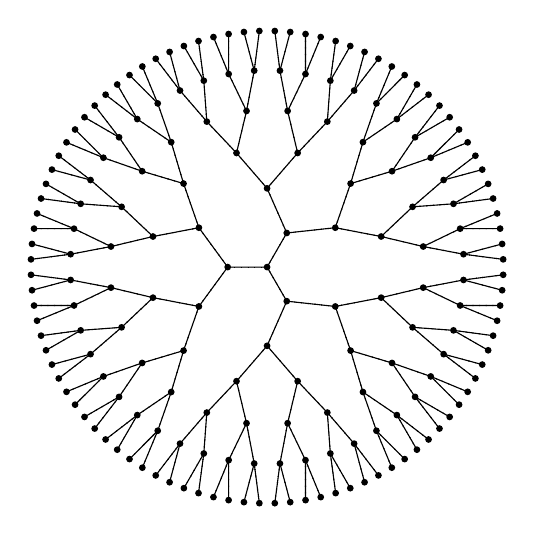
\begin{tikzpicture}[scale=0.5]
        \def\levels{6}
        \draw[fill] (0:0) circle (2pt);
        \foreach \i in {1,...,\levels} {
          \pgfmathparse{3*2^\i}
          \let\nodes\pgfmathresult
          \foreach \j in {1,3,...,\nodes} {
            \pgfmathparse{\j + (-1)^div(\j,2)}
            \let\lower\pgfmathresult
            \ifthenelse{\i = \levels}{
              \draw[dotted] (360/\nodes*\j : \i) --
              (360/\nodes*\lower : \i - 1);
            }{
              \draw[fill] (360/\nodes*\j : \i) circle (2pt) --
              (360/\nodes*\lower : \i - 1);
            }
          }
        }
      \end{tikzpicture}
      (non-CM) $2$-isogeny graph over $ℂ$
    \end{column}
  \end{columns}
\end{frame}  
  
% 9. Frobenius, diagonalisation, local structure

\begin{frame}{What happens over a finite field $\F_p$?}
  \begin{block}{Rational isogenies ($ℓ≠p$)}
    In the algebraic closure \emph{$\bar{\F}_p$}
    \[\emph{E[ℓ] = 〈P,Q〉 ≃ (ℤ/ℓℤ)^2}\]
    However, an isogeny is \emph{defined over $\F_p$} only if its kernel
    is \emph{Galois invariant}.
  \end{block}

  \begin{columns}
    \begin{column}{0.47\textwidth}
      Enter the \emph{Frobenius map}
      \begin{align*}
        π : E &→ E\\
        (x,y) &↦ (x^p,y^p)
      \end{align*}
      \emph{$E$} is seen here as a curve over \emph{$\bar{\F}_p$}.
    \end{column}
    \begin{column}{0.47\textwidth}
      \begin{block}{The Frobenius action on $E[ℓ]$}
        \begin{tikzpicture}[]
          \uncover<1>{
            \node at (0,0){$π(P) =$};   
            \node at (0,0.7){$π(Q) =$};
          }
          \node at (1.8,0){$a\uncover<-3>{P +} b\uncover<-3>{Q}$};
          \node at (1.8,0.7){$c\uncover<-3>{P +} d\uncover<-3>{Q}$};
          \uncover<3->{
            \node at (0.8,0.35){$\Biggl($}; \node at (2.7,0.35){$\Biggr)$};
          }
          \uncover<5->{
            \node at (0.3,0.35){$π:$};
            \node at (3.3,0.35){$\mod ℓ$};
          }
        \end{tikzpicture}

        \uncover<6->{We identify \emph{$π|E[ℓ]$} to a conjugacy class
          in \emph{$\GL(ℤ/ℓℤ)$}.}
      \end{block}
    \end{column}
  \end{columns}
\end{frame}

%%

\begin{frame}{What happens over a finite field $\F_p$?}
  \begin{center}
    Galois invariant subgroups of \emph{$E[ℓ]$}\\
    =\\
    eigenspaces of \emph{$π∈\GL(ℤ/ℓℤ)$}\\
    =\\
    rational isogenies of \emph{degree $ℓ$}
  \end{center}
  \pause
  \begin{block}{How many Galois invariant subgroups?}
    \begin{itemize}
    \item \emph{$π|E[ℓ] \sim \mat{λ&0\\0&λ}$}
      \hfill $→ \emph{ℓ+1}$ isogenies
    \item \emph{$π|E[ℓ] \sim \mat{λ&0\\0&μ}$} with \emph{$λ≠μ$}
      \hfill $→$ \emph{two} isogenies
    \item \emph{$π|E[ℓ] \sim \mat{λ&*\\0&λ}$}
      \hfill $→$ \emph{one} isogeny
    \item \emph{$π|E[ℓ]$} is not diagonalizable
      \hfill $→$ \emph{no} isogeny
    \end{itemize}
  \end{block}
\end{frame}

% 10. Endomorphisms, endomorphism ring, Kohel

\begin{frame}{What happens over a finite field $\F_p$?}
  \begin{block}{Endomorphisms}
    An isogeny $E→E$ is also called an \emph{endomorphism}. Examples:
    \begin{itemize}
    \item scalar multiplication \emph{$[n]$},
    \item Frobenius map \emph{$π$}.
    \end{itemize}
    With \emph{addition} and \emph{composition}, the endomorphisms
    form a ring \emph{$\End(E)$}.
  \end{block}

  \begin{block}{Theorem (Deuring)}
    \emph{$\End(E)$} is isomorphic to one of the following:
    \begin{itemize}
    \item An order $\O$ in a quadratic imaginary field $K=ℚ(\sqrt{-D})$:
      \begin{flushright}
        $E$ is \emph{ordinary} with \emph{complex multiplication} by
        $\O$.
      \end{flushright}
    \item A maximal order in a quaternion
      algebra\footnote{(ramified at $p$ and $\infty$)}:
      \begin{flushright}
        $E$ is \emph{supersingular}.
      \end{flushright}
    \end{itemize}
  \end{block}
\end{frame}

%%

\begin{frame}{Volcanology \parencite{kohel}}

  \begin{columns}
    \begin{column}{0.5\textwidth}
      Let \emph{$E,E'$} be curves with respective endomorphism rings \emph{$\O,\O'⊂K$}.\\
      Let \emph{$ϕ:E→E'$} be an isogeny of prime degree \emph{$ℓ$},
      then:
    \end{column}
    \begin{column}{0.5\textwidth}
      \centering{}
      \begin{tabular}{l l}
        if $\O=\O'$, & $ϕ$ is \emph{horizontal};\\
        if $[\O':\O]=ℓ$, & $ϕ$ is \emph{ascending};\\
        if $[\O:\O']=ℓ$, & $ϕ$ is \emph{descending}.
      \end{tabular}      
    \end{column}
  \end{columns}

  \bigskip

  \centering
  \begin{tikzpicture}
    \def\crater{7}
    \foreach \i in {1,...,\crater} {
      \draw[fill] (360/\crater*\i:1cm) circle (5pt);
      \draw (360/\crater*\i : 1cm) -- (360/\crater*\i+360/\crater : 1cm);
      \foreach \j in {-1,1} {
        \draw[fill] (360/\crater*\i : 1cm) -- (360/\crater*\i + \j*360/\crater/4 : 2cm) circle (3pt);
        \foreach \k in {-1,0,1} {
          \draw[fill] (360/\crater*\i + \j*360/\crater/4 : 2cm) --
          (360/\crater*\i + + \j*360/\crater/4 + \k*360/\crater/6 : 2.5cm) circle (1pt);
        }
      }
    }
    \begin{scope}[xshift=4cm]
      \node at (0,2) {$\End(E)$};
      \draw[fill] (0,1) circle(5pt) node[xshift=0.7cm]{$\O_K$} -- 
      (0,0) circle(3pt) --
      (0,-1) circle(1pt) node[xshift=0.7cm]{$ℤ[π]$};
    \end{scope}
  \end{tikzpicture}
  
  \small
  Ordinary isogeny volcano of degree $ℓ=3$.
\end{frame}

%%

\begin{frame}{Volcanology \parencite{kohel}}
  \centering
  \begin{columns}
    \begin{column}{0.35\textwidth}
      Let $E$ be ordinary, \emph{$\End(E)⊂K$}.

      \bigskip

      $\O_K$: \emph{maximal order} of $K$,\\
      $D_K$: \emph{discriminant} of $K$.

      \bigskip
      
      \uncover<2->{Height \emph{$= v_ℓ([\O_K:ℤ[π]])$}.}
      
      \bigskip
      
      \uncover<3->{\alert{How large is the crater?}}
    \end{column}
    \begin{column}{0.65\textwidth}
      \centering
      \begin{tikzpicture}[scale=0.8]
        \small
        \begin{scope}
          \draw[fill] (0,0) circle (2pt)
          -- (-1,-1) circle (2pt)
          (0,0) -- (0,-1) circle (2pt)
          (0,0) -- (1,-1) circle (2pt);
          \node at (0,-2) {$\left(\frac{D_K}{ℓ}\right) = -1$};
        \end{scope}    

        \begin{scope}[xshift=3.5cm]
          \draw[fill] (0,0) circle (2pt)
          -- (-0.5,-1) circle (2pt)
          (0,0) -- (0.5,-1) circle (2pt)
          (0,0) -- (2,0) circle (2pt)
          -- (1.5,-1) circle (2pt)
          (2,0) -- (2.5,-1) circle (2pt);
          \node at (1,-2) {$\left(\frac{D_K}{ℓ}\right) = 0$};
        \end{scope}
        
        \begin{scope}[xshift=2.5cm,yshift=-3cm]
          \draw[fill] (-0.8,0) node[coordinate] (A) {} circle (2pt)
          -- +(0,-1) circle (2pt)
          (0,-0.3) node[coordinate] (B) {} circle (2pt)
          -- +(0,-1) circle (2pt)
          (0.8,0) node[coordinate] (C) {} circle (2pt)
          -- +(0,-1) circle (2pt);
          \draw[bend right=20]
          (A) edge (B)
          (B) edge (C)
          (C) edge[dashed,bend right=90] (A);
          \node at (0,-2) {$\left(\frac{D_K}{ℓ}\right) = +1$};
        \end{scope}
      \end{tikzpicture}
    \end{column}  
  \end{columns}
  
  \bigskip
  
  \begin{tabular}{c | c | c c c}
    && \textbf{Horizontal} & \textbf{Ascending} & \textbf{Descending}\\
    \hline
    $\ell\nmid[\O_K:\O]]$ & $\ell\nmid[\O:ℤ[π]]$ &$1+\left(\frac{D_K}{ℓ}\right)$& &\\
    $\ell\nmid[\O_K:\O]]$ & $\ell\mid[\O:ℤ[π]]$ &$1+\left(\frac{D_K}{ℓ}\right)$& &$\ell-\left(\frac{D_K}{ℓ}\right)$\\
    $\ell\mid[\O_K:\O]]$ & $\ell\mid[\O:ℤ[π]]$ &  &$1$&$\ell$\\
    $\ell\mid[\O_K:\O]]$ & $\ell\nmid[\O:ℤ[π]]$ & &$1$& 
  \end{tabular}
\end{frame}

% 11. Tate, lighthouse, bathymeter, ℓ-adic Couveignes

\begin{frame}{Exploring isogeny graphs}
  \def\levels{6}
  \begin{columns}
    \begin{column}{0.5\textwidth}
      \begin{tikzpicture}[scale=0.5]
        \draw[fill] (0:0) circle (2pt);
        \foreach \i in {1,...,\levels} {
          \pgfmathparse{3*2^\i}
          \let\nodes\pgfmathresult
          \foreach \j in {1,3,...,\nodes} {
            \pgfmathparse{\j + (-1)^div(\j,2)}
            \let\lower\pgfmathresult
            \ifthenelse{\i = \levels}{
              \draw[dotted] (360/\nodes*\j : \i) --
              (360/\nodes*\lower : \i - 1);
            }{
              \draw[fill,black!20!white] (360/\nodes*\j : \i) circle (2pt) --
              (360/\nodes*\lower : \i - 1);
              \uncover<\i->{
                \draw[fill] (360/\nodes*\j : \i) circle (2pt) --
                (360/\nodes*\lower : \i - 1);
              }
            }
          }
        }
        \uncover<\levels->{
          \node[anchor=south] at (0,-0.5) {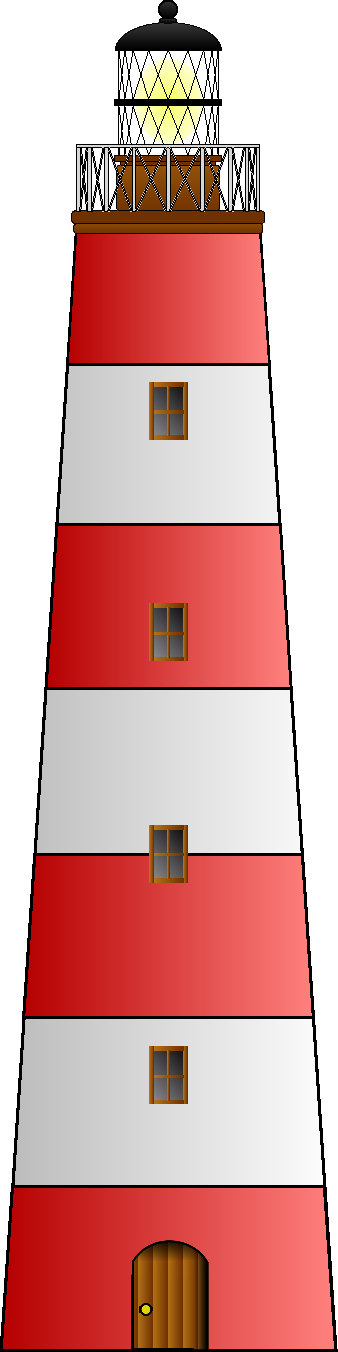
\includegraphics[height=2cm]{lighthouse}};
        }
      \end{tikzpicture}
    \end{column}
    \begin{column}{0.45\textwidth}
      Detecting the structure of a graph

      \begin{center}
        \begin{tikzpicture}
          \pgfmathparse{\levels-1}
          \let\last\pgfmathresult
          \foreach \i in {1,...,\last} {
            \uncover<\i>{
              \node at (0,0) {$π|E[ℓ^\i] \;:\;
                \begin{pmatrix}
                  a&b\\c&d
                \end{pmatrix}
                \mod ℓ^\i$};
            }
          }
          \uncover<\levels>{
            \node at (0,0) {$π|T_ℓ(E) \;:\;
              \begin{pmatrix}
                a&b\\c&d
              \end{pmatrix}
              ∈ \GL(ℤ_ℓ)$};
          }
        \end{tikzpicture}
      \end{center}

      \uncover<\levels>{
        \begin{block}{The Tate module}
          \emph{Projective limit} of the torsion:
          \[T_ℓ(E) = \varprojlim E[ℓ^n] ≃ (ℤ_ℓ)^2\]
          \bigskip
          Tate's \emph{isogeny theorem}:
          \begin{gather*}
            \Hom_{\F_p}(E,E')⊗ℤ_ℓ\\
            ≃\\
            \Hom_{\Gal(\bar{\F}_p/\F_p)}(T_ℓ(E),T_ℓ(E'))
          \end{gather*}
        \end{block}
      }
    \end{column}
  \end{columns}
\end{frame}

%%

\begin{frame}{Bathymetry}
  \begin{theorem}[\cite{defeo2016explicit}]
    Let \emph{$E/\F_p$} be an ordinary elliptic curve with Frobenius
    endomorphism~\emph{$π$}. %
    Assume that the characteristic polynomial of~\emph{$π$} has two
    distinct roots~\emph{$λ, μ$} in~\emph{$ℤ_ℓ$}, and let
    \emph{$h=v_ℓ(λ-μ)=v_ℓ(\sqrt{Δ_π/Δ_K})$}.  Then there exists a
    unique \emph{$e ∈ \{0,h\}$} such that $π|T_ℓ(E)$~is conjugate,
    over~\emph{$ℤ_ℓ$}, to the matrix \emph{$\mat{λ&ℓ^e\\0&μ}$}.
      
    Moreover, \emph{$h=v_ℓ([\O_K:ℤ[π]])$} is the height of the graph
    of \emph{$E$}; if~\emph{$E$} lies at the surface, then
    \emph{$e=h$}, otherwise \emph{$h - e$}~is the depth of~\emph{$E$}.
  \end{theorem}

  Computing \emph{$π|T_ℓ(E)$} lets us:
  \begin{itemize}
  \item Determine the height of the $ℓ$-volcano,
  \item Determine the level of $E$ in the volcano,
  \item Associate the eigenvalues $λ,μ$ to two \emph{opposite
      directions} on the crater.
  \end{itemize}

  \bigskip
  
  \emph{Application:} best known algorithm for the \emph{Explicit
    Isogeny Problem (2)}.
\end{frame}

% 12. Towers of points, towers of extensions

\begin{frame}{Computing $T_ℓ(E)$ to finite precision}
  \emph{$T_ℓ(E)$} ``modulo'' $ℓ^n$ is just \emph{$E[ℓ^n]$}:
  \[π \;:\; \mat{a&b\\c&d} \mod ℓ^n\]

  \begin{block}{Problem: fields of definitions get increasingly large}
    \begin{tabular}{c c c c c c c}
      && $E[ℓ]$ & $⊂$ & $E[ℓ^2]$ & $\dots$ & $E[ℓ^n]$\\
      && $∩$ && $∩$ && $∩$\\
      $E(\F_p)$ & $⊂$ & $E(\F_{p^{ℓ-1}})$ & $⊂$ & $E(\F_{p^{ℓ(ℓ-1)}})$ & $\dots$ & $E(\F_{p^{ℓ^{n-1}(ℓ-1)}})$
    \end{tabular}
  \end{block}
\end{frame}

% 13. Sage demo?

% 14. Perspectives in finite fields

% 15. How large is the crater? complex multiplication

% 16. PQ cartoon

\begin{frame}{Elliptic curves}
  \centering
  
\includegraphics[height=0.7\textheight]{ec-happy}
\end{frame}

%%

\begin{frame}{The QUANTOM Menace}
  \centering
  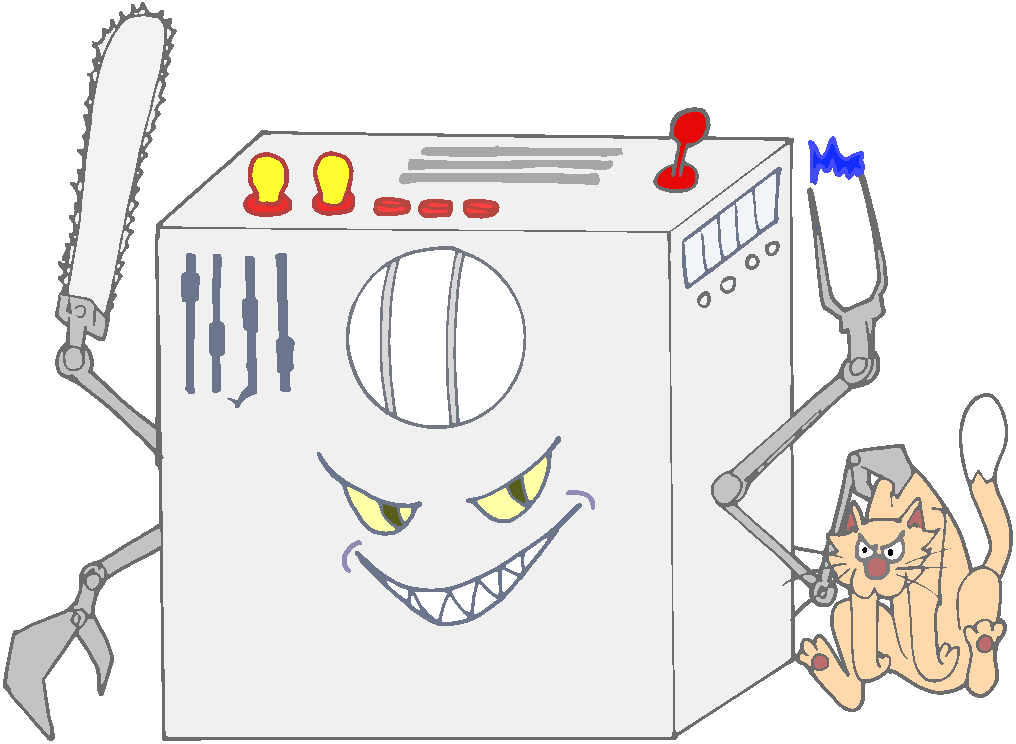
\includegraphics[height=0.7\textheight]{qc-color}
\end{frame}

%%

\begin{frame}{Post-quantum cryptographer?}
  \centering
  
\includegraphics[height=0.7\textheight]{ec-broke}
\end{frame}

%%

\begin{frame}{Elliptic curves of the world, UNITE!}
  \centering
  \begin{tikzpicture}
    \foreach \x/\y in {0/-0.5,4/2,8/-1}{
      \node at (\x,\y) {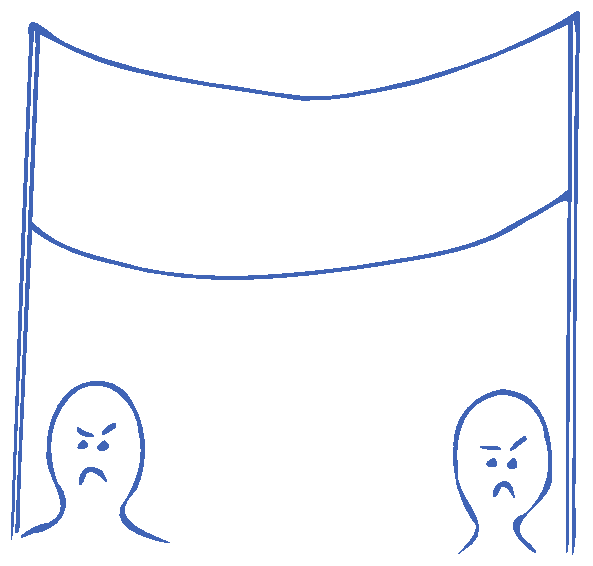
\includegraphics[height=3cm]{ec-banderole}};
    }
    \foreach \x/\y in {1/3,4.5/-1,7/3}{
      \node at (\x,\y) {
\includegraphics[height=3.5cm]{ec-sign}};
    }
    \color{teal!70!blue}\itshape\bfseries\comicneue
    \node[rotate=-3] at (5.9,3.6) {\parbox{0pt}{QUOUSQUE\\QUANTUM?}};
    \node[rotate=-3] at (3.6,-0.4) {\parbox{0pt}{QUANTUM\\SUFFICIT!}};
  \end{tikzpicture}
\end{frame}

%%

\begin{frame}{And so, they found a way around the QUANTOM}
  \centering
  \begin{tikzpicture}
    \comicneue\itshape
    \node at (0,0) {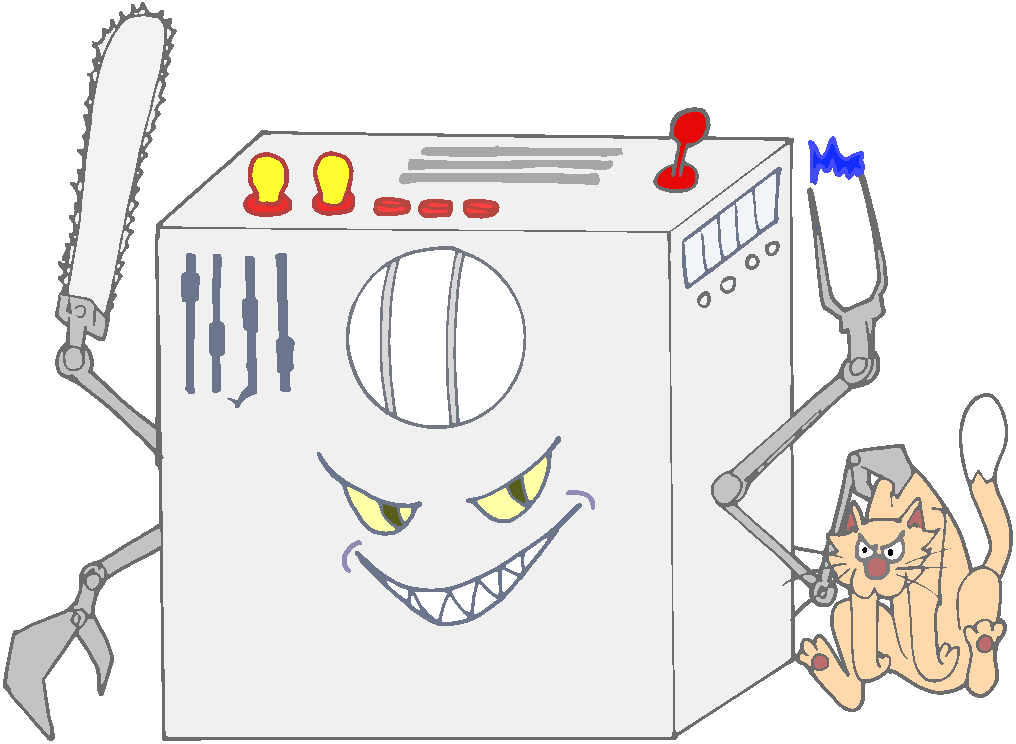
\includegraphics[height=2.5cm]{qc-color}};
    
    \node(E0) at (-5,0) {
\includegraphics[height=1cm]{ec-happy}};

    \uncover<2->{
      \node(EA) at (0,3.5) {
\includegraphics[height=1cm]{ec-happy}};
      \node(EB) at (0,-3.5) {
\includegraphics[height=1cm]{ec-happy}};
      \draw[->,decorate,decoration=snake] (E0) to (EA);
      \draw[->,decorate,decoration=snake] (E0) to (EB);
      \node[right=0.3cm of EA] {\bl{Public curve}};
      \node[right=0.3cm of EB] {\bl{Public curve}};
    }
    \uncover<3>{
      \node(ES) at (5,0) {
\includegraphics[height=1cm]{ec-happy}};
      \draw[->,decorate,decoration=snake] (EA) to (ES);
      \draw[->,decorate,decoration=snake] (EB) to (ES);
      \node[below=1em of ES] {\rd{Shared secret}};
    }
  \end{tikzpicture}
\end{frame}

% 17. CRS

{
  \newcommand{\myedge}[3]{
    \draw[#3] (360/\crater*#1 : \diam) to[bend right] (360/\crater*#2 : \diam);
  }

\begin{frame}
  \frametitle{Rostovtsev \& Stolbunov key exchange }

  \begin{columns}
    \begin{column}{0.55\textwidth}
      \begin{tikzpicture}
        \begin{scope}
          \def\crater{12}
          \def\jumpa{-8}
          \def\jumpb{9}
          \def\diam{2.5cm}
          
          \foreach \i in {1,...,\crater} {
            \pgfmathparse{int(mod(2^\i,13))}
            \let\exp\pgfmathresult
            \draw[fill] (360/\crater*\i: \diam) circle (2pt);
          }
          \uncover<2,6->{
            % Alice 1
            \myedge{0}{1}{blue}\myedge{1}{5}{red}\myedge{5}{6}{blue}\myedge{6}{3}{green}
          }
          \uncover<3,5>{
            % Bob 1
            \begin{scope}[dashed,thick]
              \myedge{0}{4}{red}\myedge{4}{8}{red}\myedge{8}{5}{green}\myedge{5}{6}{blue}
            \end{scope}
          }
          \uncover<5>{
            % Alice 2
            \myedge{6}{7}{blue}\myedge{7}{11}{red}\myedge{11}{0}{blue}\myedge{0}{9}{green}
          }
          \uncover<6->{
            % Bob 2
            \begin{scope}[dashed,thick]
              \myedge{3}{7}{red}\myedge{7}{11}{red}\myedge{11}{8}{green}\myedge{8}{9}{blue}
            \end{scope}
          }

          \draw (0 : \diam + 0.4cm) node {$E$};
          \uncover<2->{\draw (360/\crater*3 : \diam + 0.4cm) node {$\a*E$};}
          \uncover<3->{\draw (360/\crater*6 : \diam + 0.6cm) node {$\b*E$};}
          \uncover<5->{\draw (360/\crater*9 : \diam + 0.4cm) node {$\a\b*E\uncover<6->{=\b\a*E}$};}
        \end{scope}
      \end{tikzpicture}  
    \end{column}    
    \begin{column}{0.45\textwidth}
      \textbf{Public parameters:}
      \begin{itemize}
      \item A starting curve \emph{$E/\F_p$} with \emph{CM by $\O_K$};
      \item A set of ideals of small norm \emph{$S\subset\Cl(\O_K)$}.
      \end{itemize}
      \begin{enumerate}
      \item<2-> \textbf{Alice} takes a \alert{secret} random walk
        \emph{$\a=\prod_{\frak s\in S}\frak s^{e_{\frak s}}$}
        defining an isogeny \emph{$E\to \a*E$};
      \item<3-> \textbf{Bob} does the same;
      \item<4-> They publish \emph{$\a*E$} and \emph{$\b*E$};
      \item<5-> \textbf{Alice} repeats her secret walk \emph{$\a$}
        starting from \emph{$\b*E$}.
      \item<6-> \textbf{Bob} repeats his secret walk \emph{$\b$}
        starting from \emph{$\a*E$}.
      \end{enumerate}
    \end{column}
  \end{columns}
\end{frame}
}

% 18. timeline of ibc, I need a hero

% 19. Vélu to the rescue, Frobenius, CSIDH

% 20. SIDH, comparison?

\begin{frame}
  \frametitle{Key exchange with supersingular curves (2011)}
  
  \begin{description}
  \item[Good news:] there is no action of a commutative class group.
  \item[Bad news:] there is no action of a commutative class group.
  \item[Idea:] Let \bl{Alice} and \rd{Bob} walk in two
    \emph{different isogeny graphs} on the \emph{same vertex set}.
  \end{description}

  \begin{columns}
    \begin{column}{0.7\textwidth}
      \centering
      \begin{tikzpicture}[scale=1.4]
        \begin{scope}[every node/.style={fill,black,circle,inner sep=2pt}]
          \node at (0,0)  (1){};
          \node at (0,4) (20){};
          \node at (2,1)  (16z){};
          \node at (-2,1)  (81z){};
          \node at (-1,2) (77z){};
          \node at (1,2)  (20z){};
          \node at (-2,3)  (85z){};
          \node at (2,3)  (12z){};
        \end{scope}

        \begin{uncoverenv}<1,3>
          \begin{scope}[blue,every loop/.style={looseness=50}]
            \path (1) edge (20) edge (16z) edge (81z);
            \path (20) edge[loop left] (20) edge[loop right] (20);
            \path (16z) edge (81z) edge (77z);
            \path (81z) edge (20z);
            \path (77z) edge (20z) edge (85z);
            \path (20z) edge (12z);
            \path (12z) edge[bend right=10] (85z) edge[bend left=10] (85z);
          \end{scope}
        \end{uncoverenv}
        
        \begin{uncoverenv}<2->
          \begin{scope}[red]
            \path (1) edge (85z) edge (81z) edge (12z) edge (16z);
            \path (20) edge (85z) edge (77z) edge (20z) edge (12z);
            \path (81z) edge (85z) edge (77z) edge (16z);
            \path (85z) edge (12z);
            \path (12z) edge (16z);
            \path (16z) edge (20z);
            \path (20z) edge[bend right=10] (77z) edge[bend left=10] (77z);
          \end{scope}
        \end{uncoverenv}
      \end{tikzpicture}
    \end{column}
    \begin{column}{0.3\textwidth}
      \small
      \emph{Figure:} \bl{$2$}- and \rd{$3$}-isogeny graphs on $\F_{97^2}$.
    \end{column}
  \end{columns}
\end{frame}

%%

\begin{frame}
  \frametitle{Key exchange with supersingular curves}

  \begin{itemize}
  \item Fix small primes \bl{$\ell_A$}, \rd{$\ell_B$};
  \item \emph{No canonical labeling} of the \bl{$\ell_A$}- and
    \rd{$\ell_B$}-isogeny graphs; \emph{however\dots}
  \end{itemize}

  \begin{center}
    \bf
    Walk of length \bl{$e_A$}\\
    $=$\\
    Isogeny of degree \bl{$\ell_A^{e_A}$}\\
    $=$\\
    Kernel \bl{$\langle P\rangle\subset E[\ell_A^{e_A}]$}
  \end{center}
  
  \begin{center}
    \begin{tikzpicture}
      \begin{scope}
        \draw (0,1.2) node[anchor=east,blue] {$\ker\phi=〈P〉\subset E[\ell_A^{e_A}]$};
        \draw (0,0.4) node[anchor=east,red] {$\ker\psi=〈Q〉\subset E[\ell_B^{e_B}]$};
        \draw (0,-0.4) node[anchor=east,blue] {$\ker\phi' = 〈\rd{\psi}(P)〉$};
        \draw (0,-1.2) node[anchor=east,red] {$\ker\psi' = 〈\bl{\phi}(Q)〉$};
      \end{scope}
      \begin{scope}[xshift=4.5cm,coils/.style={-angle 90,decorate,decoration={coil,aspect=0,amplitude=1pt}}]
        \large
        \node[matrix of nodes, ampersand replacement=\&, column sep=3cm, row sep=1.5cm] (diagram) {
          |(E)| $E$ \& |(Es)| $E/〈\bl{P}〉$ \\
          |(Ep)| {$E/〈\rd{Q}〉$} \& |(Eps)| {$E/〈\bl{P},\rd{Q}〉$}\\
        };
        \path[->,blue] (E) edge[coils] node[auto] {$\phi$} (Es);
        \path[->,blue] (Ep) edge[coils] node[auto,swap] {$\phi'$} (Eps);
        \path[->,red] (E) edge[coils] node[auto,swap] {$\psi$} (Ep);
        \path[->,red] (Es) edge[coils] node[auto] {$\psi'$} (Eps);
      \end{scope}
    \end{tikzpicture}
  \end{center}
\end{frame}

% 21. Perspectives (signature, etc.)

%%


\end{document}


% LocalWords:  Isogeny abelian isogenies hyperelliptic supersingular Frobenius
% LocalWords:  isogenous isogeny


